\chapter{Propozycja rozwiązania}

\section{Tworzenie aplikacji od podstaw}
\label{nowa_aplikacja}
Jak już autor wspomniał w rozdziale \ref{test_driven_development} dotyczącym metodologii TDD, wytwarzanie oprogramowania zaczynając od testowania powoduje, że zostanie napisanie tylko tyle aplikacji, ile to jest ujęte w wymaganiach. A co za tym idzie jej stopień komplikacji zostanie ograniczony do niezbędnego minimum.

\textit{i tutaj sięgamy do książeczki i piszemy o TDD}

\section{Nowe podejście do architektury systemu}
\label{clean_architecture}
Największą przeszkodą w testowaniu aplikacji androidowych jest niestety sam Android. Im większy \textit{coupling} między warstwami, tym trudniej jest pisać testy jednostkowe. Rozważmy więc przekształcenie modelu aplikacji Android opisanego na początku poprzedniego rozdziału w następujący sposób:

\begin{figure}[!htb]
    \centering
    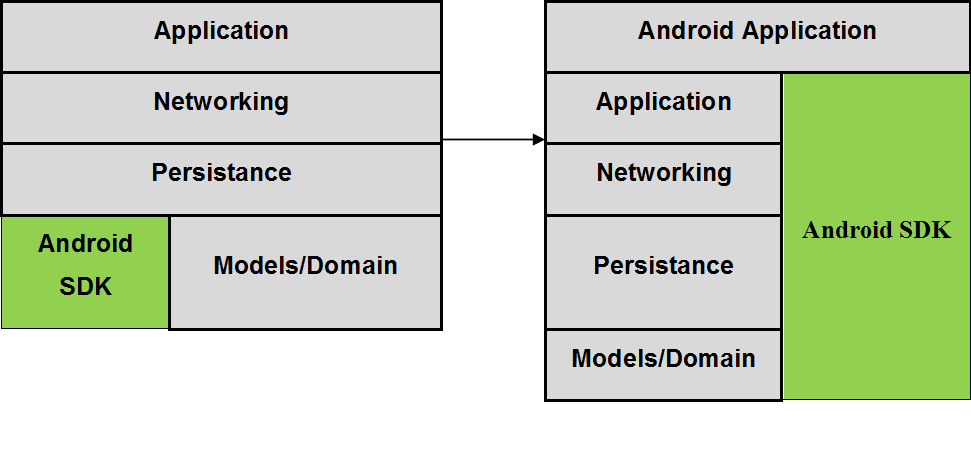
\includegraphics[width=13cm]{imgs/ch4_opis_rozwiazania_1.png}
    \caption
{Zmodyfikowana struktura aplikacji Android: Clean Architecture}
    \label{fig:opis_rozwiazania}
\end{figure} 

Nowy model aplikacji oddziela (przynajmniej w teorii) warstwy Application, Networking, Persistance oraz Model/Domain od środowiska Android SDK, a co za tym idzie nie musimy umieszczać odwołania do tego środowiska praktycznie w każdym pliku (wyrażenie \texttt{import android.*}). Dopiero najwyższą warstwą jest warstwa Aplikacja Android. W takim podejściu staramy się użyć Androida jako pewnego rodzaju \textit{pluginu} do naszej aplikacji i uniezależnić warstwę logiczną od reszty warstw. Czyli najpierw napiszemy aplikację, która będzie oddzielona od Android SDK (na przykład w czystej Javie), potem dołączymy do tego android SDK i złączymy to wszystko w Aplikację Android. W ten sposób zapewnimy, że kod, który stanowi podstawę naszej aplikacji, czyli jej logikę działania, był przetestowany tak jak należy, czyli w oddzieleniu od reszty warstw.

Robert Cecil Martin \footnote{Robert Cecil Martin (Uncle Bob) to amerykański inżynier programista oraz autor książek o programowaniu. Jest również współautorem „Agile manifesto”}, znany szerzej w środowisku informatycznym jako Uncle Bob, opublikował w 2012 roku na swoim blogu propozycję usystematyzowania kodu Android. Schemat przedstawiony jest na poniższym rysunku:

\begin{figure}[!htb]
    \centering
    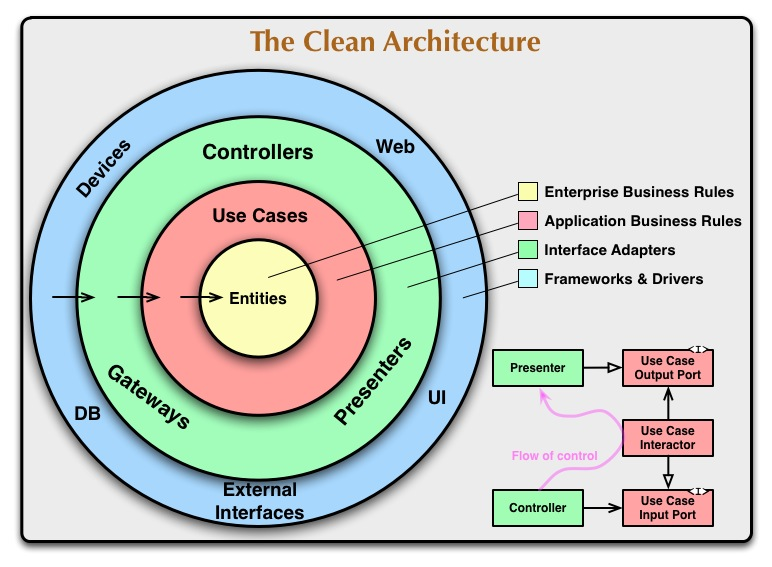
\includegraphics[width=13cm]{imgs/ch4_clean_architecture.jpg}
    \caption
{Clean architecture of Android według Uncle Ben. Źródło: http://blog.8thlight.com/uncle-bob/2012/08/13/the-clean-architecture.html}
    \label{fig:clean architecture}
\end{figure} 

Idea tego schematu jest następująca:

\begin{itemize}

\item
Najważniejszym elementem jest środek, czyli warstwa \textit{Entities}. W warstwie tej znajdują się kluczowe dla tworzonej aplikacji reguły biznesowe gwarantujące poprawność działania programu. Krótko mówiąc – znajduje się tam logika działania aplikacji.
\item
Drugą warstwą są \textit{Use Cases}. W wolnym tłumaczeniu są to przypadki użycia, ale lepiej chyba używać nazwy intencje biznesowe. Jest to zbiór wszystkich zachowań, jakich oczekujemy od tworzonego systemu. W przypadku aplikacji bankowej, może być to na przykład funkcja wykonywania przelewu, jako jeden \textit{use case}, a innym przypadkiem użycia byłoby sprawdzenie stanu konta.
\item
Wyższa, otaczająca warstwa dotyczy wszystkich kontrolerów i prezenterów. Warto zauważyć, że nadal na tym etapie nie mamy powiązania z systemem Android.
\item
Dopiero na ostatniej, najbardziej zewnętrznej warstwie pojawia nam się powiązanie z Android SDK. Korzystamy z niego aby dostać się do baz danych, skorzystać z interfejsów użytkownika dla danego urządzenia, uzyskać dostęp do zewnętrznych interfejsów lub urządzeń.
\end{itemize}

I teraz rzecz najważniejsza: pomiędzy warstwami na schemacie narysowane są strzałki, które informują nas o kierunku przekazywania informacji. Ze schematu wynika, że \textit{Entities} nie wiedzą nic o istnieniu \textit{Use Cases}, \textit{Use Cases} nie posiadają informacji o kontrolerach i prezenterach, a te z kolei nie wiedzą o istnieniu interfejsu użytkownika. Patrząc w drugą stronę, każda warstwa wyższa posiada wszystkie informacje o warstwie niższej, czyli UI wie wszystko o prezenterach, te wiedzą wszystko o \textit{Use Cases}, no i przypadki użycia mogą korzystać z całej warstwy logicznej.

Przekładając to na język języków programowania, jeżeli używamy instrukcji \texttt{import android.*}, to tylko w stosunku do wyższej warstwy. Nie wolno nam tego robić w stosunku do warstwy niższej, bo wtedy cała koncepcja zostanie zachwiana.

W ten sposób teoretycznie jesteśmy w stanie stworzyć architekturę, która:
\begin{itemize}
\item
jest niezależna od frameworka (tutaj Android SDK) – i zachowujemy zasadę zależności,
\item
jest niezależna od UI, bazy danych lub innych urządzeń zewnętrznych,
\item
jest testowalna, w oderwaniu od warstwy zawierającej interfejsy wymienione powyżej, czyli od wszystkiego, co czyni testy na Androidzie trudnymi.
\end{itemize}

Jeżeli ułożymy naszą strukturę aplikacji w powyższy sposób – testowanie powinno odbywać się jak w przypadku kodu napisanego w czystej Javie czy C++.

\section{Praca z kodem zastanym}
\label{legacy_code}
W rozdziale \ref{pielegnowalnosc_aplikacji} nawiązaliśmy już do problemu pracy z kodem zastanym, tak zwanym \textit{Legacy Code}.
Co więc zrobić, aby zaimplementować testy do już napisanego kodu? Godfrey Nolan\footnote{Godfrey Nolan - założyciel i prezes RIIS LLC, firmy zajmującej się rozwojem oprogramowania dla platform przenośnych. Autor książek o Androidzie: "Agile Android", "Booletproof android", "Android Best Practices" i "Decompiling Android"} w swojej książce "Agile Android"\cite{bib:agile:android} proponuje następujące rozwiązanie:

\begin{itemize}
\item 
Wprowadzić metodę ciągłej integracji w procesie budowania kodu -  (\textit{Continuous Integration (CI)}).

Jest to należąca do metodologii zwinnych praktyka polegająca na regularniej integracji zmian w kodzie do bieżącego repozytorium. Warunkiem koniecznym umieszczenia kodu w repozytorium jest upewnienie się, że dany kod działa.

\item
Przy projektowaniu nowych funkcjonalności używać metody TDD.

\item
Skorzystać z serwera CI (dobrym przykładem jest tutaj \textit{Jenkins}\footnote{http://jenkins-ci.org/}), który będzie wykonywał unit testy, do których mamy przekonanie, że ich implementacja nie powinna się zmieniać. Oczywiście tylko na tym etapie, bo testy automatyczne muszą również podlegać przeglądom.

\item
Uświadomić zespół programistów na czym polegają testy jednostkowe i przekonać ich do stosowania TDD.

\item
Dodać metryki mierzenia kodu do CI. Ustawić poziom minimalny na 10-15\%.

\item
Użyć frameworka do podstawowych testów GUI już istniejącej aplikacji (najlepiej \textit{Espresso}). Stworzyć testy opierając się na przypadkach użycia (ang. \textit{use cases)}.

\item
Bezwzględnie pisać testy jednostkowe do nowych części oprogramowania zgodnie z TDD, \textit{mockując} jeśli to możliwe wykorzystywane obiekty z zastanego kodu.

\item
Wyizolować zastany kod, tak aby nikt z programistów nie miał do niego dostępu, jeżeli naprawdę nie musi.

\item
Usunąć niewykorzystywane i nieużyteczne części kodu.

\item
Przepisać i przetestować wyizolowany kod, aby zwiększyć metryki pokrycia do około 60-70\%. 
\end{itemize}

Najważniejsze więc jest wyizolować stary kod, przetestować aplikację za pomocą frameworka do testów GUI, usunąć ewentualne błędy niepozwalające na poprawną pracę programu i nie modyfikować wyizolowanego kodu podczas pisania nowych funkcjonalności. Nowe funkcje należy dodawać stosując już TDD. Dopiero na końcu, jeżeli nasze środowisko jest już stabilne, należy rozpocząć przebudowę starych części aplikacji, tak aby metryki pokrycia kodu rosły wraz z upływem czasu. Przy wykonywaniu \textit{refaktoringu} Godfrey Nolan proponuje użyć narzędzia SonarQube\footnote{SonarQube - platforma do prowadzenia ciągłej inspekcji jakości kodu źródłowego, dostarczana na licencji \textit{open source}}.